\documentclass[pmlr]{jmlr}% PMLR format (Deep Learning Indaba / JMLR-PMLR guidelines)
% jmlr auto-loads: amsmath, amssymb, natbib, graphicx, url, algorithm2e.

\usepackage{booktabs}
\usepackage{float}
\usepackage{tcolorbox}
\usepackage{tikz}
\usetikzlibrary{positioning,shapes.geometric,arrows.meta,calc}
\graphicspath{{figures/}}
\newcommand{\acc}{\mathrm{Acc}}

\jmlrvolume{}
\jmlryear{2026}
\jmlrworkshop{Trustworthy AI Workshop, Deep Learning Indaba 2026}

% Remove the first-page copyright footer, and the running header on pages 2+.
\makeatletter
\renewcommand*{\@titlefoot}{}
\makeatother

\title[Confidently Wrong: Appendix]{Confidently Wrong: Measuring and Mitigating Calibration Risks in LLMs for African Languages \\[2pt] \large Supplementary Appendix}

% Anonymized for double-blind review.
\author{\Name{Anonymous Author(s)}}

\begin{document}

\maketitle
\thispagestyle{jmlrtps}% keep the PMLR line on page 1
\pagestyle{plain}% no running header on pages 2+ (page numbers only)
\vspace{-2.2em}

\noindent\textit{This appendix accompanies the anonymous submission ``Confidently Wrong: Measuring
and Mitigating Calibration Risks in LLMs for African Languages'' and is provided as a separate file,
in compliance with the Trustworthy AI Workshop (Deep Learning Indaba 2026) submission guidelines.
Section, table, and figure numbers refer to this appendix; ``the main paper'' refers to the
accompanying extended abstract.}

\appendix

\section{Models}\label{app:models}
\begin{table}[H]\centering\small
\caption{Open-weight models evaluated.}
\label{tab:models}
\resizebox{\textwidth}{!}{%
\begin{tabular}{llll}
\toprule
\textbf{Model} & \textbf{Params} & \textbf{Type} & \textbf{Hugging Face ID}\\
\midrule
Qwen3-4B-Instruct & 4B  & Instruction-tuned & \texttt{Qwen/Qwen3-4B-Instruct}\\
Gemma-4-12B       & 12B & Instruction-tuned & \texttt{google/gemma-4-12b-it}\\
Aya-Expanse-8B    & 8B  & Multilingual      & \texttt{CohereLabs/aya-expanse-8b}\\
AfroLlama-V1      & 7B  & Africa-specific (LLaMA-2 base) & \texttt{Jacaranda/AfroLlama\_V1}\\
\bottomrule
\end{tabular}}
\end{table}

AfroLlama-V1 is based on LLaMA-2-7B and was fine-tuned on Swahili, Zulu, Yoruba, Hausa, Xhosa, and
English; Amharic and N.\,Sotho, which appear in our benchmarks, are out-of-distribution for this
model. All models are loaded in \texttt{bfloat16} with scaled dot-product (\texttt{sdpa}) attention,
a 2048-token context limit, and greedy decoding (temperature 0), on a single NVIDIA A100 (40\,GB).

\section{Metric definitions}\label{app:metrics}
For an item with options $o$ and gold answer $y$, the cloze score of option $o$ with tokens
$o_1,\dots,o_L$ given context $x$ is the length-normalised log-probability
\begin{equation}
s(o) = \frac{1}{L}\sum_{t=1}^{L}\log p(o_t \mid x, o_{<t}).
\end{equation}
\begin{equation}
p(o) = \operatorname{softmax}_o s(o),
\qquad \hat{y}=\arg\max_o p(o), \qquad c=\max_o p(o).
\end{equation}
Over $N$ items with correctness $y_i\in\{0,1\}$, confidence $c_i$, and $B=15$ equal-width confidence
bins $\{B_b\}$:
\begin{equation}
\mathrm{ECE}=\sum_{b=1}^{B}\frac{|B_b|}{N}\,\bigl|\acc(B_b)-\mathrm{conf}(B_b)\bigr| .
\end{equation}
\begin{equation}
\text{Overconfidence}=\frac{1}{N}\sum_i c_i-\frac{1}{N}\sum_i y_i .
\end{equation}
\begin{equation}
\text{Brier}=\frac{1}{N}\sum_i (c_i-y_i)^2 .
\end{equation}
AUROC is the area under the ROC curve using $c$ to rank correct against incorrect items. AUARC is the
area under the accuracy-rejection curve: items are answered most-confident-first and accuracy on the
answered subset is integrated over coverage. Temperature scaling rescales the logits by a single
$T>0$, $p_T(o)=\operatorname{softmax}_o\!\big(s(o)/T\big)$; we fit $T^\star=\arg\min_T \mathrm{ECE}$
on a seeded 50\% calibration split and report ECE on the held-out half.

\section{Prompts}\label{app:scoring}
Each option is scored as a continuation of the prompt; the prompt lists no answer letters.

\begin{tcolorbox}[colback=blue!4,colframe=blue!45,title=\textbf{Uhura-TruthfulQA (truthfulness)},fonttitle=\small,boxrule=0.5pt]
\ttfamily\small Q: \{question\}\\ A:
\end{tcolorbox}

\begin{tcolorbox}[colback=blue!4,colframe=blue!45,title=\textbf{AfriMMLU (knowledge)},fonttitle=\small,boxrule=0.5pt]
\ttfamily\small The following is a multiple-choice question about \{subject\}. Give the correct answer.\\[3pt]
Question: \{question\}\\ Answer:
\end{tcolorbox}

For 5-shot prompting, the prompt is prefixed with five solved examples in the same language, each
formatted as the template above followed by its gold answer text and separated by blank lines; the
examples are held out from evaluation.

\section{Interventions}\label{app:interventions}
By \emph{interventions} we mean lightweight, post-hoc procedures applied at or after inference to
improve calibration or to trade answer coverage for reliability, without any retraining of the model.
We evaluate three:
\begin{enumerate}\itemsep1pt
  \item \textbf{Temperature scaling.} We fit one temperature $T$ per language by minimising ECE on a
  seeded 50\% calibration split and evaluate on the held-out half, searching the grid
  $T \in \{0.5, 0.6, 0.7, 0.8, 0.9, 1.0, 1.2, 1.5, 2.0, 3.0, 5.0\}$.
  \item \textbf{Selective abstention.} The model answers only when its calibrated confidence exceeds
  a per-language threshold chosen from the risk-coverage curve; we report AUARC integrated over all
  coverage levels.
  \item \textbf{Few-shot prompting.} Five in-context examples per language, drawn from held-out items,
  formatted identically to the evaluation prompt and prepended to each query.
\end{enumerate}

\section{Deployment framework}\label{app:framework}
Figure~\ref{fig:framework} translates our findings into a deployment policy for African-language
LLMs. The model's raw confidence is first recalibrated by per-language temperature scaling; the
calibrated confidence $\hat{c}$ is then compared against two per-language thresholds. High-confidence
queries ($\hat{c}\geq\tau_{\mathrm{hi}}$) are answered, medium-confidence queries trigger a request
for more context and a re-query, and low-confidence queries ($\hat{c}<\tau_{\mathrm{lo}}$) are
abstained on or deferred to a human; all low-confidence queries are logged to guide future
African-language data collection.

\begin{figure}[htbp]\centering
\resizebox{0.95\textwidth}{!}{%
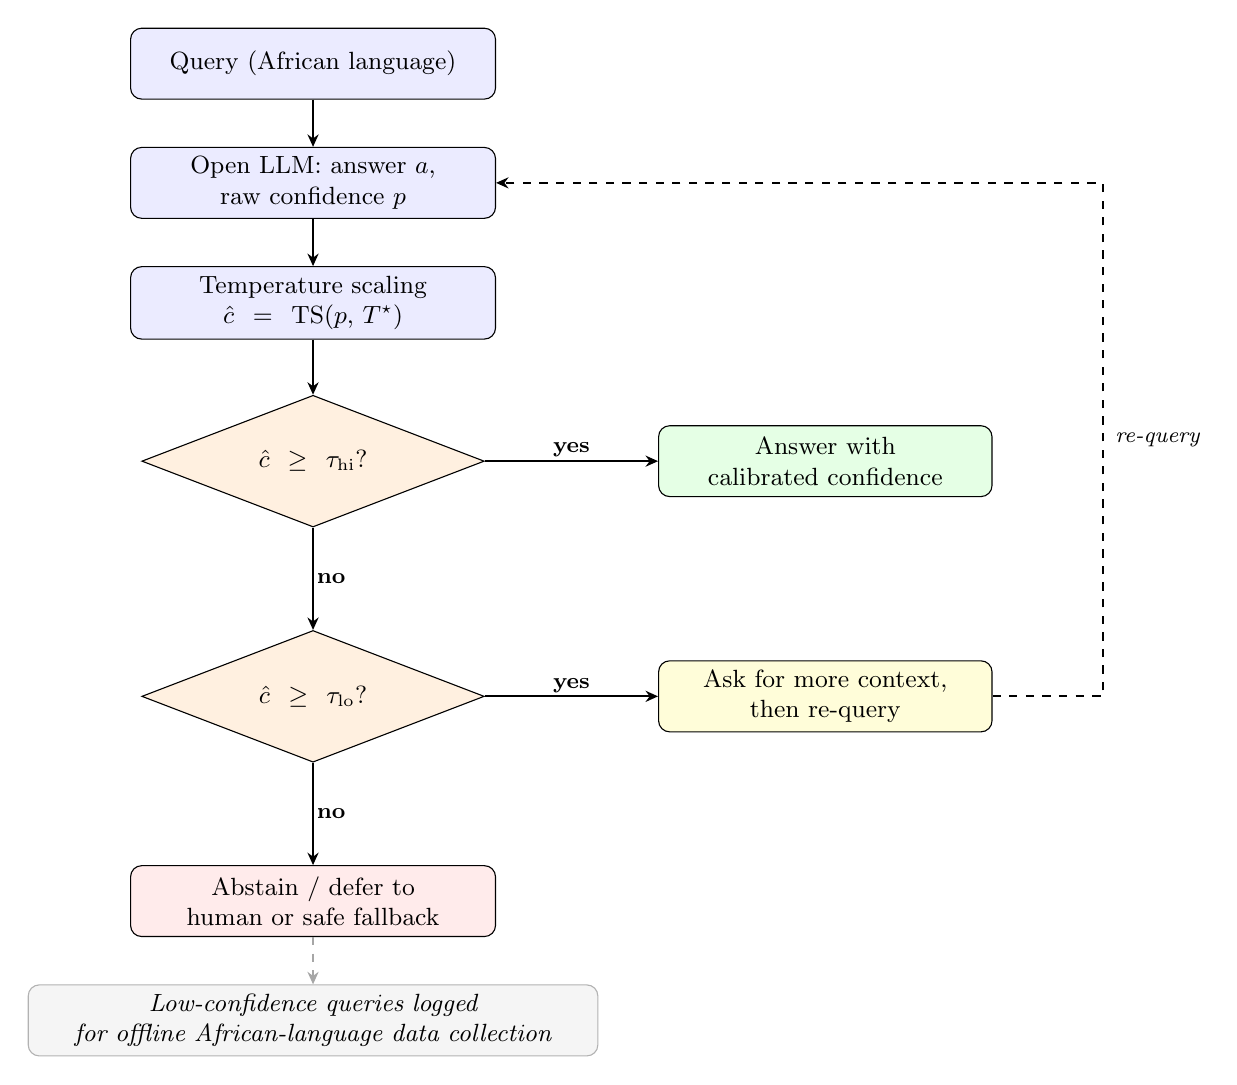
\begin{tikzpicture}[
  node distance  = 6mm,
  every node/.style = {font=\small},
  proc/.style    = {rectangle, rounded corners=4pt, draw, fill=blue!8,
                    text width=44mm, align=center, minimum height=9mm},
  dec/.style     = {diamond, draw, fill=orange!12, aspect=2.6,
                    text width=34mm, align=center, inner sep=1pt},
  outbox/.style  = {rectangle, rounded corners=4pt, draw,
                    text width=40mm, align=center, minimum height=9mm},
  logrect/.style = {rectangle, rounded corners=4pt, draw=gray!60,
                    fill=gray!8, text width=70mm, align=center,
                    minimum height=9mm, font=\small\itshape},
  arr/.style     = {-{Stealth[length=4.5pt,width=4pt]}, thick},
  lbl/.style     = {font=\footnotesize\bfseries, inner sep=1pt},
]
\node[proc]                   (q)   {Query (African language)};
\node[proc, below=of q]       (llm) {Open LLM: answer $a$,\\ raw confidence $p$};
\node[proc, below=of llm]     (ts)  {Temperature scaling\\ $\hat{c} = \mathrm{TS}(p,\,T^\star)$};
\node[dec,  below=7mm of ts]  (d1)  {$\hat{c} \geq \tau_{\mathrm{hi}}$?};
\node[dec,  below=13mm of d1] (d2)  {$\hat{c} \geq \tau_{\mathrm{lo}}$?};
\node[proc, below=13mm of d2, fill=red!8] (abs) {Abstain / defer to\\ human or safe fallback};
\node[logrect, below=6mm of abs] (log) {Low-confidence queries logged\\for offline African-language data collection};
\node[outbox, fill=green!10, right=22mm of d1] (ans) {Answer with\\ calibrated confidence};
\node[outbox, fill=yellow!15, right=22mm of d2] (ctx) {Ask for more context,\\ then re-query};
\draw[arr] (q)   -- (llm);
\draw[arr] (llm) -- (ts);
\draw[arr] (ts)  -- (d1);
\draw[arr] (d1)  -- node[lbl,right]{no} (d2);
\draw[arr] (d2)  -- node[lbl,right]{no} (abs);
\draw[arr, dashed, gray!70] (abs) -- (log);
\draw[arr] (d1.east) -- node[lbl,above]{yes} (ans.west);
\draw[arr] (d2.east) -- node[lbl,above]{yes} (ctx.west);
\draw[arr, dashed]
  (ctx.east)
    -- ++(14mm, 0) coordinate (RightA)
    -- (RightA |- llm.east)  coordinate (RightB)
    -- (llm.east);
\node[font=\footnotesize\itshape, right=1pt] at ($(RightA)!0.5!(RightB)$) {re-query};
\end{tikzpicture}}
\caption{Deployment framework for LLMs in African languages. Recalibrate first with per-language
temperature scaling, then route on calibrated confidence $\hat{c}$: high values
($\hat{c}\geq\tau_{\mathrm{hi}}$) are answered with the stated confidence; medium values trigger a
request for more context followed by re-query; low values ($\hat{c}<\tau_{\mathrm{lo}}$) are
abstained or deferred to a human or safe fallback. Thresholds $\tau$ are set per language from the
risk-coverage curve, and low-confidence queries are logged to drive offline African-language data
collection.}
\label{fig:framework}
\end{figure}

\section{Additional results}\label{app:figs}

\begin{table}[H]\centering\small
\caption{Per-language accuracy and ECE on Uhura-TruthfulQA (zero-shot). Each cell shows Acc\,/\,ECE;
\textbf{bold} ECE exceeds the English baseline for that model. $\dagger$ out-of-distribution for
AfroLlama-V1.}
\label{tab:uhura_lang}
\begin{tabular}{lcccc}
\toprule
\textbf{Language} & \textbf{AfroLlama-V1} & \textbf{Aya-Expanse-8B} & \textbf{Gemma-4-12B} & \textbf{Qwen3-4B}\\
\midrule
English (eng)               & 0.292\,/\,0.177 & 0.358\,/\,0.075 & 0.329\,/\,0.212 & 0.381\,/\,0.072\\
\midrule
Amharic (amh)$\dagger$      & 0.294\,/\,0.101 & 0.302\,/\,0.077 & 0.274\,/\,\textbf{0.293} & 0.373\,/\,0.042\\
Hausa (hau)                 & 0.363\,/\,0.085 & 0.302\,/\,\textbf{0.235} & 0.397\,/\,\textbf{0.223} & 0.308\,/\,\textbf{0.199}\\
N.\,Sotho (nso)$\dagger$    & 0.246\,/\,\textbf{0.307} & 0.260\,/\,\textbf{0.293} & 0.379\,/\,\textbf{0.232} & 0.270\,/\,\textbf{0.262}\\
Swahili (swa)               & 0.341\,/\,0.122 & 0.314\,/\,\textbf{0.215} & 0.328\,/\,\textbf{0.273} & 0.335\,/\,\textbf{0.157}\\
Yoruba (yor)                & 0.371\,/\,0.072 & 0.351\,/\,\textbf{0.141} & 0.329\,/\,\textbf{0.256} & 0.310\,/\,\textbf{0.150}\\
Zulu (zul)                  & 0.337\,/\,0.122 & 0.319\,/\,\textbf{0.237} & 0.343\,/\,\textbf{0.266} & 0.324\,/\,\textbf{0.204}\\
\bottomrule
\end{tabular}
\end{table}

\begin{table}[H]\centering\small
\caption{Per-language accuracy and ECE on AfriMMLU (zero-shot), representative subset. Each cell
shows Acc\,/\,ECE; \textbf{bold} ECE exceeds the English baseline for that model.}
\label{tab:afrimmlu_lang}
\begin{tabular}{lcccc}
\toprule
\textbf{Language} & \textbf{AfroLlama-V1} & \textbf{Aya-Expanse-8B} & \textbf{Gemma-4-12B} & \textbf{Qwen3-4B}\\
\midrule
English (eng) & 0.356\,/\,0.225 & 0.520\,/\,0.057 & 0.296\,/\,0.311 & 0.526\,/\,0.062\\
\midrule
Amharic (amh) & 0.258\,/\,0.147 & 0.240\,/\,\textbf{0.114} & 0.268\,/\,\textbf{0.314} & 0.286\,/\,\textbf{0.084}\\
Hausa (hau)   & 0.294\,/\,0.190 & 0.308\,/\,\textbf{0.172} & 0.308\,/\,\textbf{0.309} & 0.304\,/\,\textbf{0.141}\\
Swahili (swa) & 0.294\,/\,0.188 & 0.312\,/\,\textbf{0.151} & 0.280\,/\,\textbf{0.325} & 0.312\,/\,\textbf{0.139}\\
Yoruba (yor)  & 0.290\,/\,0.192 & 0.300\,/\,\textbf{0.154} & 0.250\,/\,\textbf{0.349} & 0.308\,/\,\textbf{0.126}\\
Zulu (zul)    & 0.310\,/\,0.171 & 0.292\,/\,\textbf{0.173} & 0.252\,/\,\textbf{0.362} & 0.286\,/\,\textbf{0.167}\\
Ewe (ewe)     & 0.244\,/\,\textbf{0.239} & 0.274\,/\,\textbf{0.211} & 0.252\,/\,\textbf{0.374} & 0.288\,/\,\textbf{0.175}\\
Igbo (ibo)    & 0.252\,/\,\textbf{0.245} & 0.262\,/\,\textbf{0.214} & 0.288\,/\,\textbf{0.329} & 0.258\,/\,\textbf{0.202}\\
French (fra)  & 0.280\,/\,\textbf{0.268} & 0.442\,/\,\textbf{0.071} & 0.244\,/\,\textbf{0.383} & 0.372\,/\,\textbf{0.114}\\
\bottomrule
\end{tabular}
\end{table}

\begin{table}[H]\centering\small
\caption{Per-language temperature scaling on Uhura-TruthfulQA for AfroLlama-V1 and Qwen3-4B.
$T^\star$ is selected on the calibration half; ECE values are on the held-out half.}
\label{tab:temp_scaling}
\begin{tabular}{lcccccc}
\toprule
 & \multicolumn{3}{c}{\textbf{AfroLlama-V1}} & \multicolumn{3}{c}{\textbf{Qwen3-4B}}\\
\cmidrule(lr){2-4}\cmidrule(lr){5-7}
\textbf{Language} & $T^\star$ & ECE(bef) & ECE(aft) & $T^\star$ & ECE(bef) & ECE(aft)\\
\midrule
English   & 5.0 & 0.175 & 0.069 & 1.5 & 0.096 & 0.074\\
Amharic   & 5.0 & 0.115 & 0.038 & 1.2 & 0.056 & 0.043\\
Hausa     & 2.0 & 0.085 & 0.077 & 5.0 & 0.203 & 0.027\\
N.\,Sotho & 5.0 & 0.307 & 0.093 & 5.0 & 0.260 & 0.067\\
Swahili   & 2.0 & 0.160 & 0.074 & 3.0 & 0.182 & 0.043\\
Yoruba    & 1.5 & 0.078 & 0.064 & 5.0 & 0.133 & 0.062\\
Zulu      & 2.0 & 0.126 & 0.046 & 5.0 & 0.191 & 0.085\\
\midrule
\textit{Pooled} & n/a & 0.143 & 0.036 & n/a & 0.151 & 0.030\\
\bottomrule
\end{tabular}
\end{table}

\begin{table}[H]\centering\small
\caption{Zero-shot versus 5-shot calibration on Uhura-TruthfulQA (values shown as zero-shot
$\rightarrow$ 5-shot, macro-averaged over languages). Few-shot gives small gains for three models and
backfires on Gemma-4-12B.}
\label{tab:fewshot}
\begin{tabular}{lccc}
\toprule
\textbf{Model} & \textbf{Accuracy} & \textbf{ECE} & \textbf{Overconfidence}\\
\midrule
Qwen3-4B-Instruct & $0.329 \rightarrow 0.355$ & $0.155 \rightarrow 0.141$ & $0.151 \rightarrow 0.130$\\
AfroLlama-V1      & $0.320 \rightarrow 0.339$ & $0.141 \rightarrow 0.119$ & $0.137 \rightarrow 0.113$\\
Aya-Expanse-8B    & $0.315 \rightarrow 0.331$ & $0.182 \rightarrow 0.171$ & $0.179 \rightarrow 0.164$\\
Gemma-4-12B       & $0.340 \rightarrow 0.305$ & $0.251 \rightarrow 0.332$ & $0.250 \rightarrow 0.331$\\
\bottomrule
\end{tabular}
\end{table}

\begin{figure}[htbp]\centering
  \begin{minipage}{0.49\textwidth}\centering
    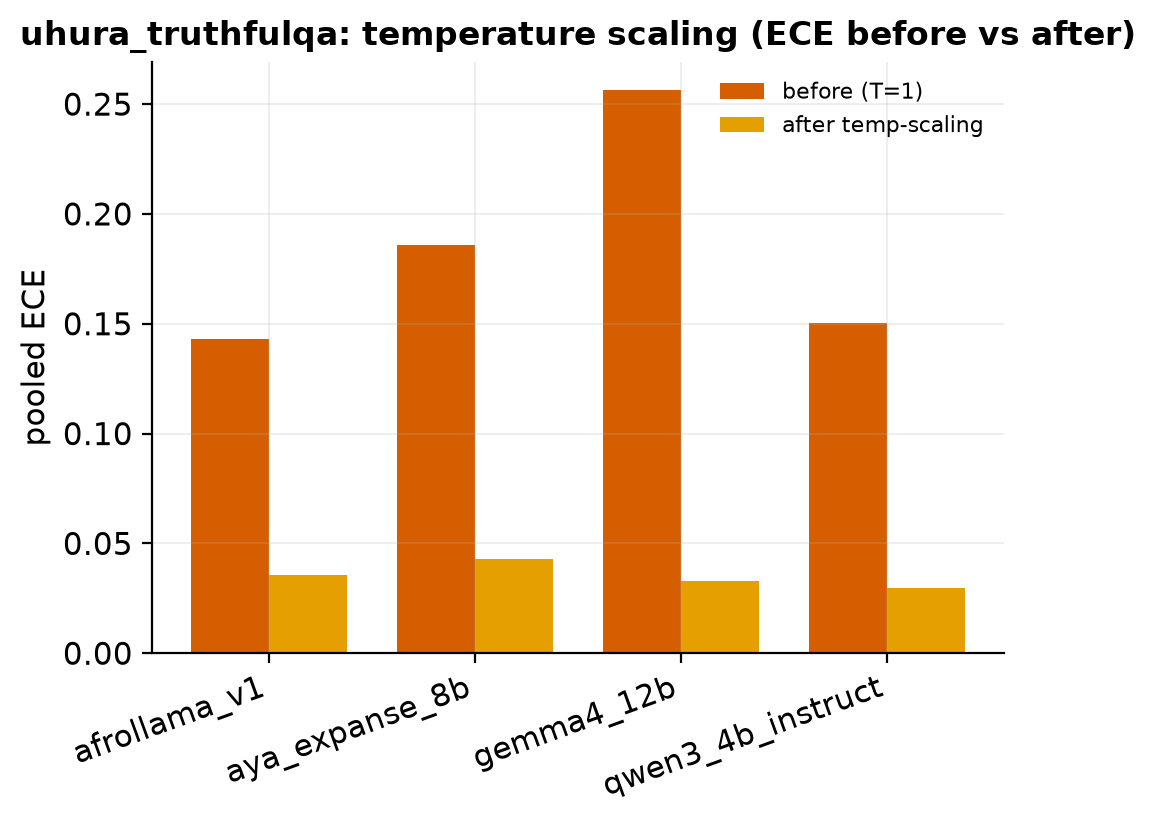
\includegraphics[width=\linewidth]{uhura_temperature_scaling.png}\\[2pt]{\small (a) Uhura-TruthfulQA}
  \end{minipage}\hfill
  \begin{minipage}{0.49\textwidth}\centering
    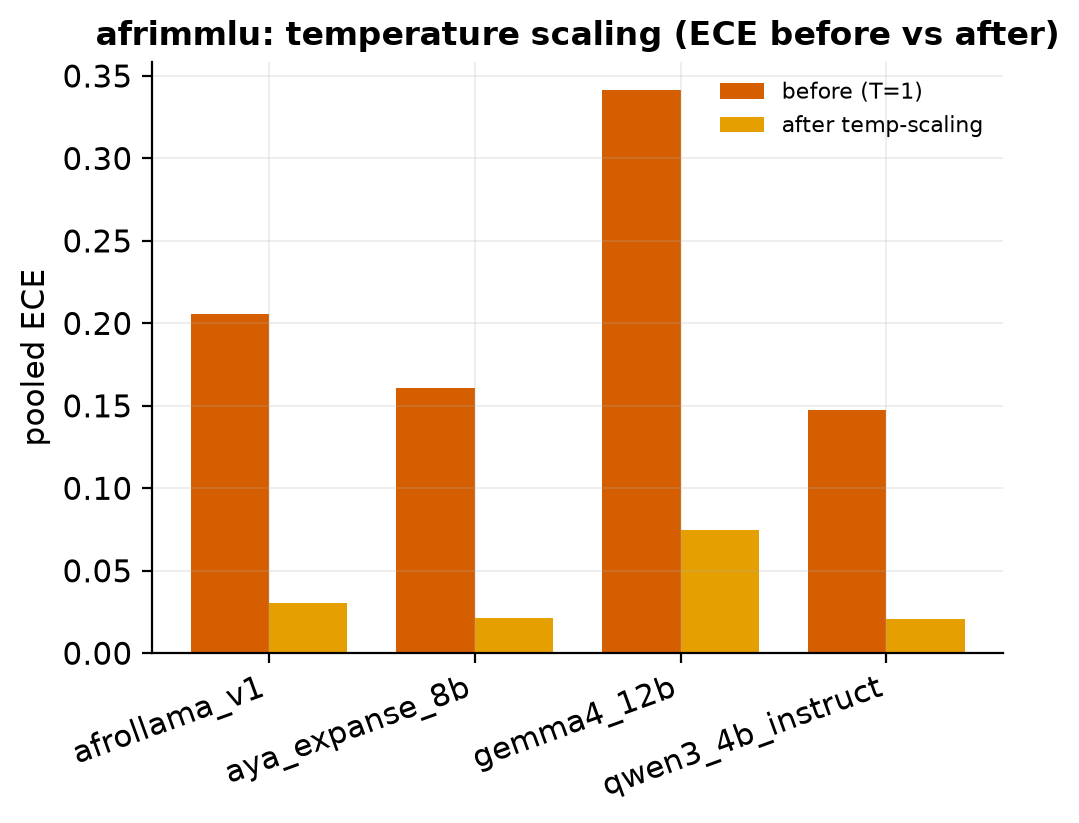
\includegraphics[width=\linewidth]{afrimmlu_temperature_scaling.png}\\[2pt]{\small (b) AfriMMLU}
  \end{minipage}
  \caption{Pooled ECE before versus after per-language temperature scaling; ECE drops to about 0.03
  for all models on both datasets.}
  \label{fig:tempscale}
\end{figure}

\begin{figure}[htbp]\centering
  \begin{minipage}{0.49\textwidth}\centering
    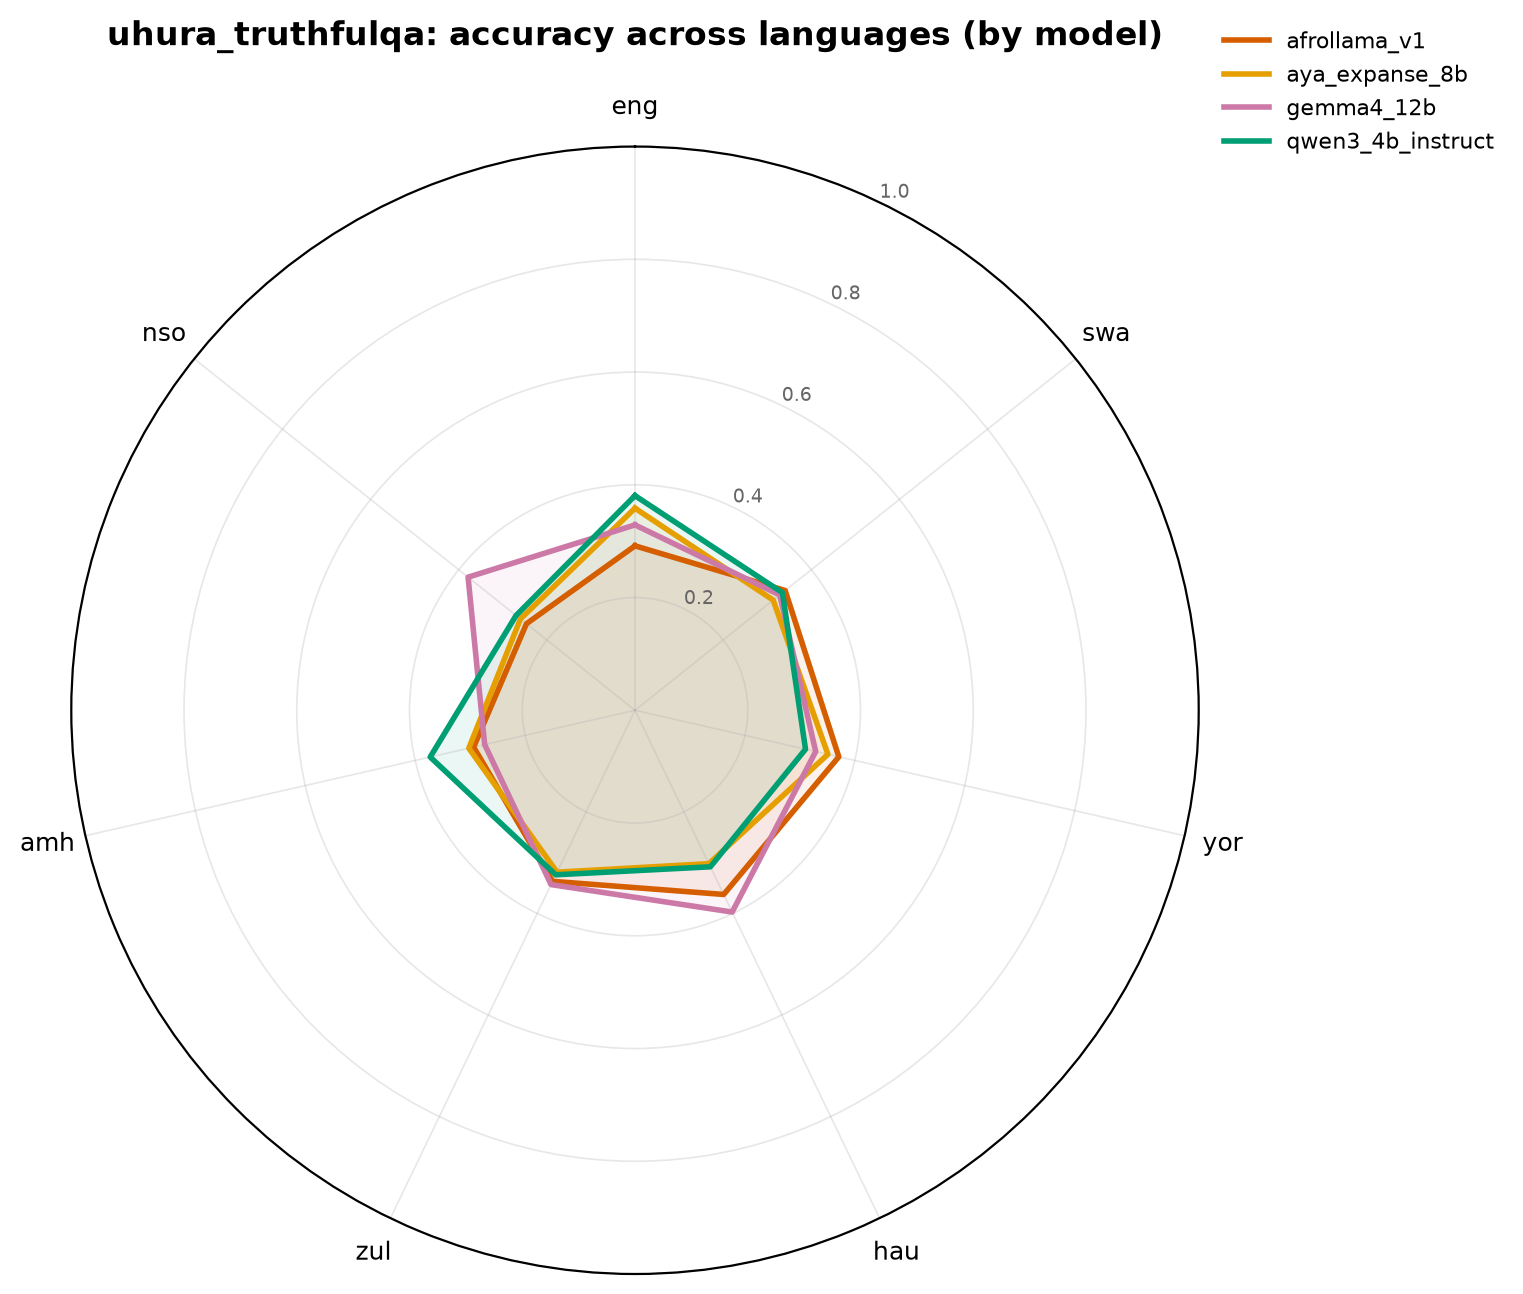
\includegraphics[width=\linewidth]{uhura_accuracy_radar.png}\\[2pt]{\small (a) Uhura-TruthfulQA accuracy by language}
  \end{minipage}\hfill
  \begin{minipage}{0.49\textwidth}\centering
    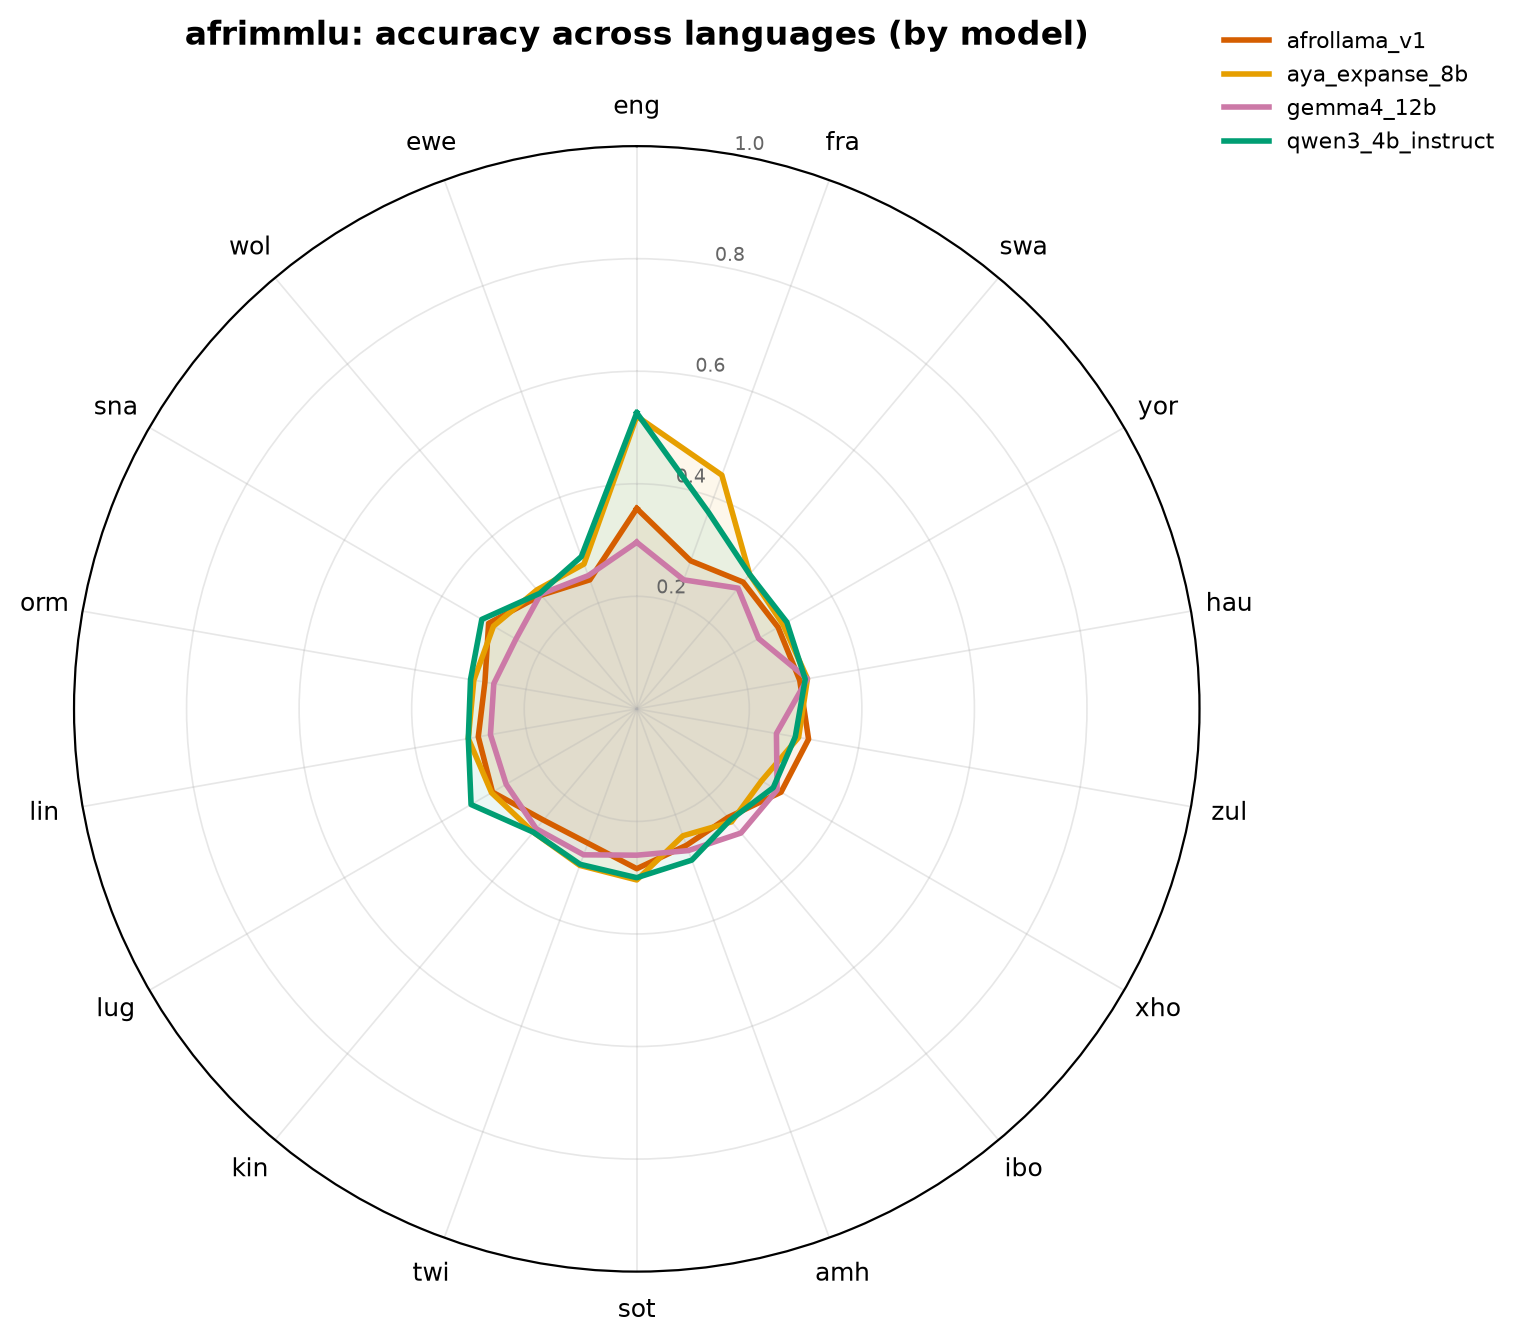
\includegraphics[width=\linewidth]{afrimmlu_accuracy_radar.png}\\[2pt]{\small (b) AfriMMLU accuracy by language}
  \end{minipage}
  \caption{Accuracy across languages by model. Long English and French spokes collapse toward chance
  across African languages.}
  \label{fig:decay}
\end{figure}

\begin{figure}[htbp]\centering
  \begin{minipage}{0.49\textwidth}\centering
    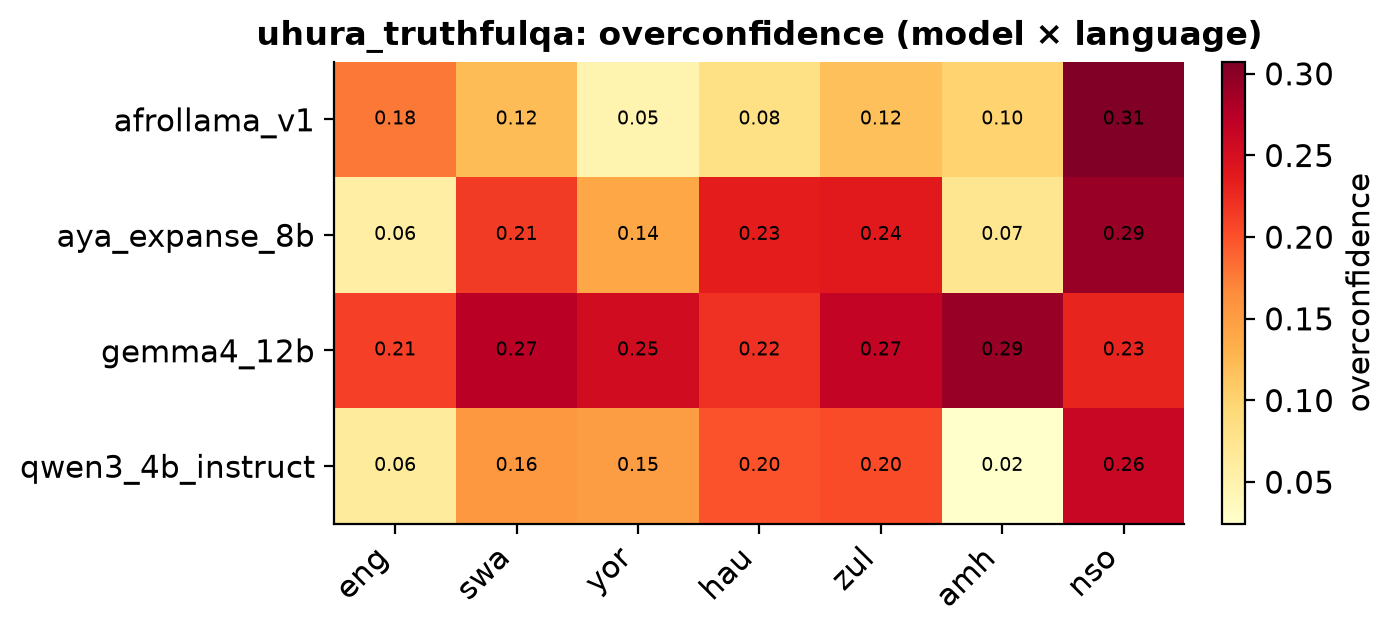
\includegraphics[width=\linewidth]{uhura_overconfidence_heatmap.png}\\[2pt]{\small (a) Uhura-TruthfulQA overconfidence by language}
  \end{minipage}\hfill
  \begin{minipage}{0.49\textwidth}\centering
    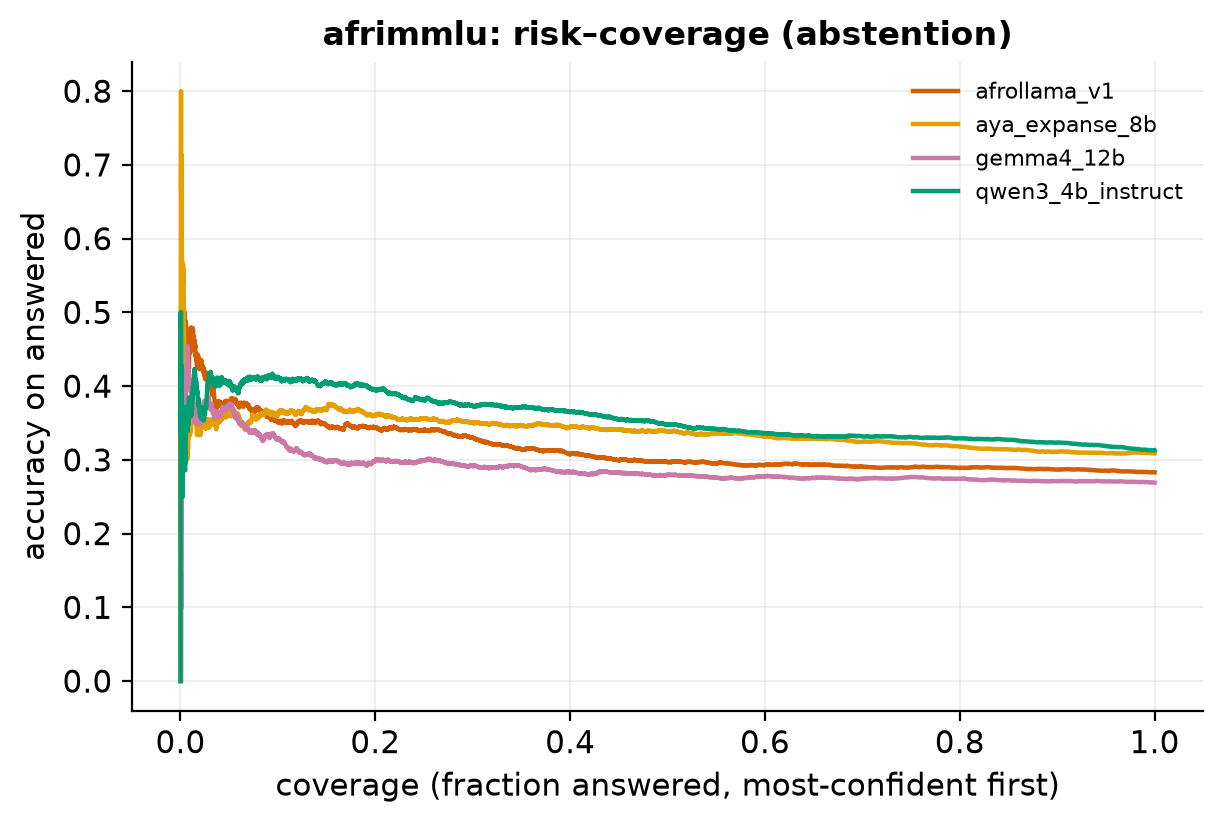
\includegraphics[width=\linewidth]{afrimmlu_risk_coverage.png}\\[2pt]{\small (b) AfriMMLU risk-coverage (abstention)}
  \end{minipage}
  \caption{Overconfidence by language (left) and the accuracy-rejection trade-off under selective
  abstention (right); AUARC sits only modestly above baseline, reflecting a weak uncertainty signal
  (AUROC about 0.55).}
  \label{fig:appextra}
\end{figure}

\begin{figure}[htbp]\centering
  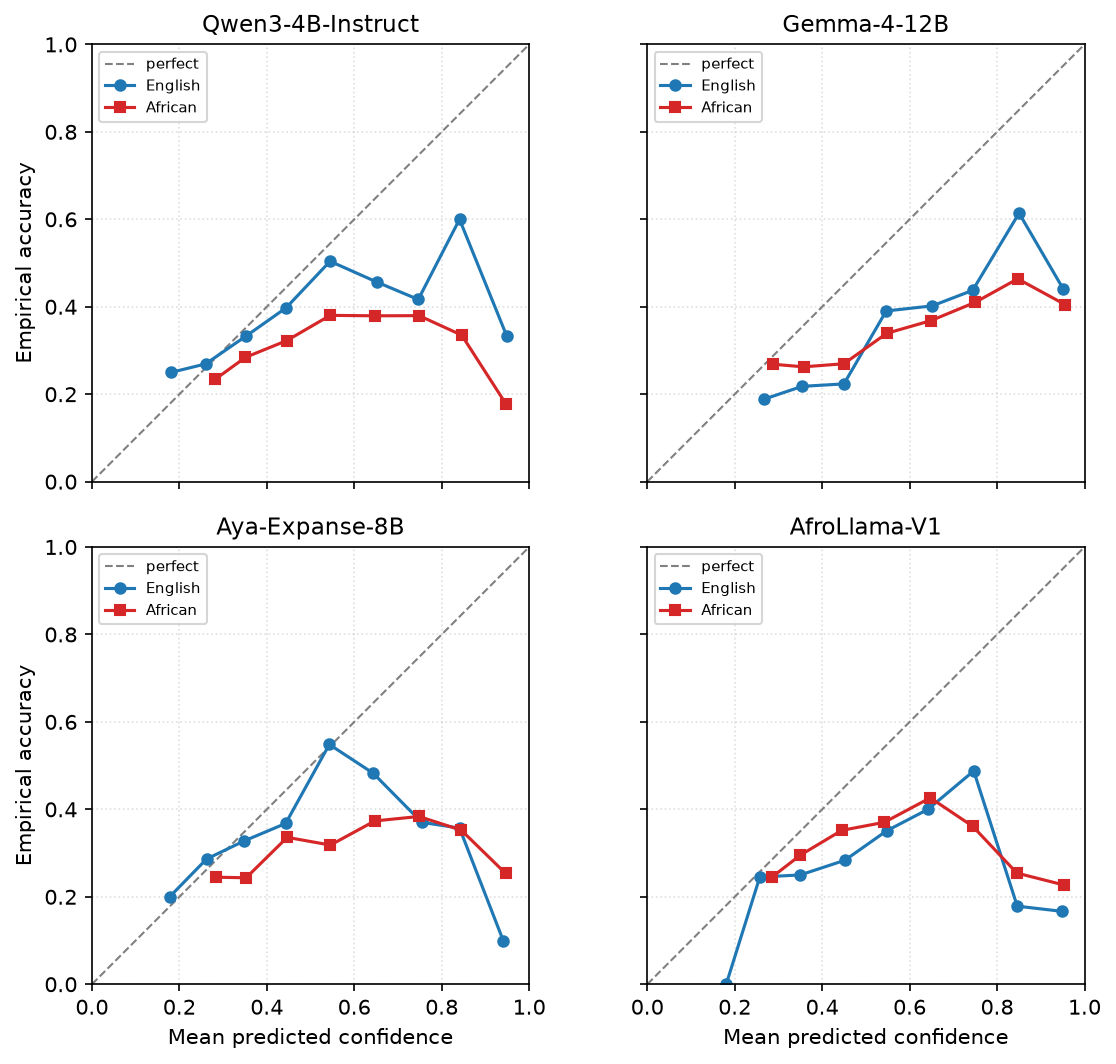
\includegraphics[width=0.82\textwidth]{uhura_reliability.png}
  \caption{Reliability curves on Uhura-TruthfulQA, English versus African languages, for each model
  (10 confidence bins). Points on the diagonal are perfectly calibrated; points below it indicate
  overconfidence. The African curve sits further below the diagonal than the English curve for the
  general-purpose models.}
  \label{fig:reliability}
\end{figure}

\section{Bootstrap confidence intervals}\label{app:bootstrap}
Table~\ref{tab:bootstrap_ci} reports 95\% bootstrap confidence intervals (2{,}000 draws, stratified
by language, fixed seed 42) for the four primary point estimates in Table~1 of the main paper. For
each model and dataset we split items into English and African subsets, group by language, and
macro-average per-language ECE and accuracy. Each bootstrap draw resamples items with replacement
within each language stratum, recomputes the per-language metrics, and macro-averages; the interval
is the 2.5th to 97.5th percentile of the resulting distribution. Because the point estimates here are
macro-averaged across languages, they can differ by up to about 0.004 from the pooled values in
Table~1 of the main paper.

\begin{table}[H]\centering\small
\setlength{\tabcolsep}{4pt}
\caption{Bootstrap 95\% confidence intervals for ECE and accuracy (zero-shot, 2{,}000 draws,
stratified by language, seed 42). Each cell shows the point estimate [lower, upper].}
\label{tab:bootstrap_ci}
\resizebox{\textwidth}{!}{%
\begin{tabular}{llcccc}
\toprule
\textbf{Model} & \textbf{Dataset} & \textbf{ECE(en)} & \textbf{ECE(afr)} & \textbf{Acc(en)} & \textbf{Acc(afr)}\\
\midrule
Qwen3-4B       & Uhura-TruthfulQA & 0.072 [0.060, 0.113] & 0.169 [0.160, 0.186] & 0.381 [0.347, 0.413] & 0.320 [0.306, 0.333]\\
Gemma-4-12B    & Uhura-TruthfulQA & 0.212 [0.182, 0.245] & 0.257 [0.246, 0.273] & 0.329 [0.297, 0.362] & 0.342 [0.328, 0.355]\\
Aya-Expanse-8B & Uhura-TruthfulQA & 0.075 [0.062, 0.114] & 0.199 [0.187, 0.214] & 0.358 [0.326, 0.392] & 0.308 [0.295, 0.321]\\
AfroLlama-V1   & Uhura-TruthfulQA & 0.177 [0.148, 0.212] & 0.135 [0.126, 0.151] & 0.292 [0.261, 0.325] & 0.325 [0.312, 0.339]\\
\midrule
Qwen3-4B       & AfriMMLU & 0.062 [0.052, 0.116] & 0.150 [0.147, 0.165] & 0.526 [0.482, 0.572] & 0.300 [0.290, 0.310]\\
Gemma-4-12B    & AfriMMLU & 0.311 [0.273, 0.354] & 0.344 [0.335, 0.355] & 0.296 [0.258, 0.336] & 0.268 [0.259, 0.277]\\
Aya-Expanse-8B & AfriMMLU & 0.057 [0.048, 0.113] & 0.173 [0.170, 0.189] & 0.520 [0.476, 0.564] & 0.296 [0.286, 0.306]\\
AfroLlama-V1   & AfriMMLU & 0.225 [0.187, 0.267] & 0.207 [0.201, 0.219] & 0.356 [0.312, 0.398] & 0.279 [0.269, 0.288]\\
\bottomrule
\end{tabular}}
\end{table}

\begin{figure}[htbp]\centering
  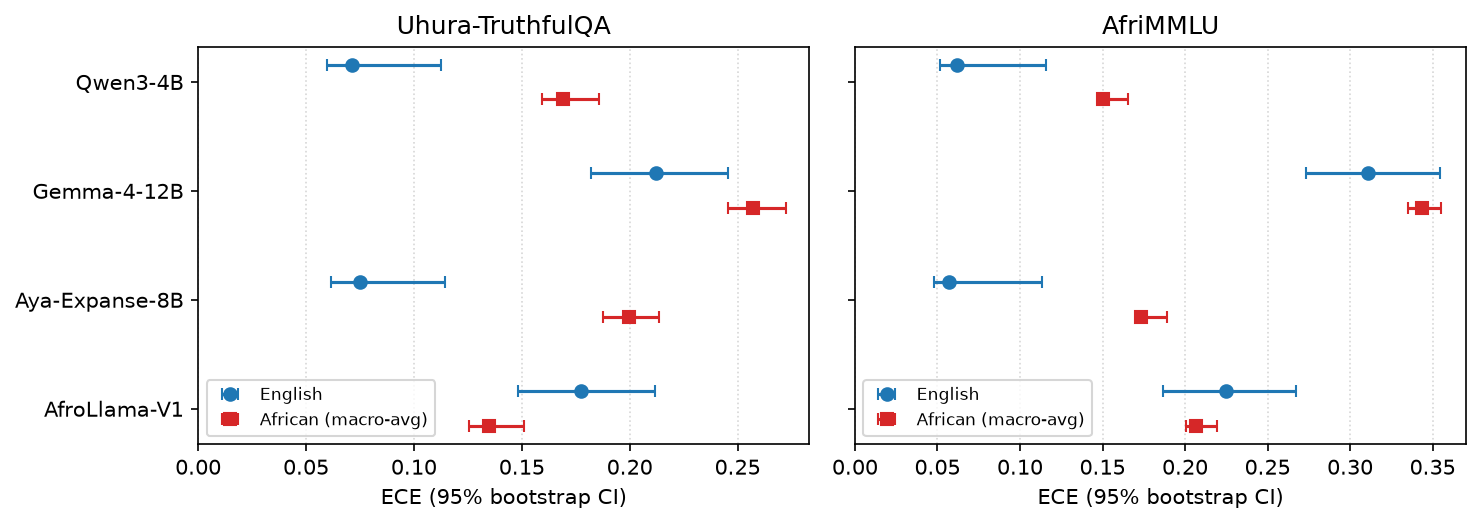
\includegraphics[width=0.8\textwidth]{bootstrap_ci.png}
  \caption{Bootstrap 95\% confidence intervals for ECE by model, English versus African languages
  (markers are point estimates, bars are 95\% intervals). For the general-purpose models the African
  interval lies entirely to the right of (above) the English interval; the intervals are disjoint.}
  \label{fig:bootstrap}
\end{figure}

English ECE intervals are wider because English is a single-language stratum, whereas African ECE is
macro-averaged over many languages, which reduces bootstrap variance.

\section{Reproducibility}\label{app:repro}
All code, predictions, figures, and tables will be released in an anonymized public repository upon
acceptance. The benchmarks used are publicly available: \path{masakhane/uhura-truthfulqa} and
\path{masakhane/afrimmlu}.

\section{LLM Usage}\label{app:llm}
Claude Code was used to assist with implementing and debugging the evaluation pipeline. The research
ideas, methodology, experimental design, and interpretation of results were conceptualized by the
authors. All generated code, analyses, and reported results were reviewed and verified by the
authors.

\end{document}
